\documentclass[11pt]{article}

\usepackage[a4paper,margin=27mm]{geometry}
\usepackage{fontspec}
\usepackage{xeCJK}
\usepackage{unicode-math}
\setmainfont{TeX Gyre Termes}
\setsansfont{TeX Gyre Heros}
\setmonofont{TeX Gyre Cursor}
\setmathfont{TeX Gyre Termes Math}
\setCJKmainfont{Noto Serif CJK SC}
\setCJKsansfont{Noto Sans CJK SC}
\setCJKmonofont{Noto Sans Mono CJK SC}
\usepackage{microtype}
\usepackage{amsthm}
\usepackage{amsmath}
\usepackage{booktabs}
\usepackage{tabularx}
\usepackage{array}
\usepackage{enumitem}
\usepackage{graphicx}
\usepackage{tikz}
\usetikzlibrary{arrows.meta,positioning,fit,calc,backgrounds,shapes.geometric}
\usepackage{placeins}
\usepackage{float}
\usepackage[numbers,sort&compress]{natbib}
\usepackage{xcolor}
\usepackage{url}
\usepackage{hyperref}
\usepackage[nameinlink,noabbrev]{cleveref}

\hypersetup{
  unicode=true,
  pdftitle={Technical Note: Gauge-Trivial Circle Twists and Constant-Diagonal Corona Records for Indiscrete Real Actions},
  pdfauthor={AUTHOR TO CONFIRM},
  pdfsubject={Technical note on typed circle twists, support transfer, component isometries, and a generic constant-diagonal corona lemma},
  pdfkeywords={technical note, continuous multipliers, twisted convolution, indiscrete action groupoids, gauge equivalence, support transfer, corona algebras},
  colorlinks=true,
  linkcolor=blue!45!black,
  citecolor=green!35!black,
  urlcolor=blue!55!black
}

\setlength{\parindent}{1.35em}
\setlength{\parskip}{0.23em}
\setlength{\emergencystretch}{3em}
\setlist{nosep,leftmargin=2em}
\renewcommand{\arraystretch}{1.16}
\newcolumntype{Y}{>{\raggedright\arraybackslash}X}
\newcolumntype{P}[1]{>{\raggedright\arraybackslash}p{#1}}

\newtheorem{theorem}{Theorem}[section]
\newtheorem{proposition}[theorem]{Proposition}
\newtheorem{lemma}[theorem]{Lemma}
\newtheorem{corollary}[theorem]{Corollary}
\theoremstyle{definition}
\newtheorem{definition}[theorem]{Definition}
\newtheorem{remark}[theorem]{Remark}

\newcommand{\R}{\mathbb R}
\newcommand{\Z}{\mathbb Z}
\newcommand{\T}{\mathbb T}
\newcommand{\C}{\mathbb C}
\newcommand{\Gactual}{G_{\mathrm{actual}}}
\newcommand{\Gstd}{G_{\mathrm{std}}}
\newcommand{\Qbare}{Q^{\mathrm{bare}}}
\newcommand{\Qactual}{Q_p^{\mathrm{actual}}}
\newcommand{\Qdisc}{Q_p^{\mathrm{disc}}}
\newcommand{\Std}{\operatorname{Std}}
\newcommand{\supp}{\operatorname{supp}}
\newcommand{\dist}{\operatorname{dist}}
\newcommand{\id}{\operatorname{id}}
\newcommand{\Cor}{\operatorname{Cor}}
\newcommand{\Ad}{\operatorname{Ad}}
\newcommand{\cstarmax}{C^*_{\max}}
\newcommand{\cstarred}{C^*_{\mathrm r}}
\newcommand{\AuthorConfirm}{\textbf{AUTHOR TO CONFIRM}}
\newcommand{\TraceRef}[1]{(trace artifact \nolinkurl{#1}; package README,
``Strict six-key artifact traces'')}

\title{\textbf{Technical Note: Gauge-Trivial Circle Twists and\\
Constant-Diagonal Corona Records for Indiscrete Real Actions}}
\author{\AuthorConfirm\\
\small Author list, order, affiliations, and correspondence: AUTHOR TO CONFIRM}
\date{15 August 2026}

\begin{document}
\maketitle

\begin{center}
\fbox{\begin{minipage}{0.91\linewidth}
\centering
\textbf{Article type and retained disposition: Technical Note --- NOTE branch.}
\texttt{STANDALONE\_PASS=false}.  This document does not claim a standalone
classification or an owner-specific corona obstruction.
\end{minipage}}
\end{center}

\begin{abstract}
This Technical Note concerns continuous circle twists on author records of
globally indiscrete real actions and their same-carrier standard comparison;
it is not a standalone classification.  Real-line multiplier triviality and
the twisted-convolution, gauge, amenability, $c_0$-sum, multiplier, and corona
mechanisms are prior or standard.  Companion Papers 2, 8, 9, 11, and 12
respectively supply the continuum lower bound; the one-orbit proxy and
trace/return boundary; the actual packet, topology, stabilizer, and period;
the untwisted actual records; and all-degree factorization, standardization,
and the comparison map.  At a fixed normalization, we verify the
time/actual gauge bridge and give a direct sign-exact real-line
trivialization.  We then construct separately typed twisted test, maximal,
and reduced author records with oriented gauge covariance.  Exactly four
registered outputs become constant after tags are forgotten, while literal
stabilizers, topology, and periods remain.  Actual-to-standard function
pullback has an exact support formula and a zero/finite/infinite criterion.
On each standard component, the selected time images are separately
isometric for maximal and reduced norms.  Only after those isometries is the
corona statement invoked: it is a generic constant-diagonal lemma for an
arbitrary $c_0$-sum.  Its fixed-prime instances hold for both completions but
do not distinguish or recover the prime.  Finite deterministic checks remain
diagnostics.  No topology transfer, globally named actual twisted groupoid
$C^*$-algebra, trace, determinant, or spectral promotion is obtained.
\end{abstract}

\noindent\textbf{Keywords:} continuous multipliers; twisted convolution;
indiscrete action groupoids; gauge equivalence; support transfer; corona
algebras.

\begin{center}
\textbf{中文摘要}
\end{center}
\begingroup\small
\noindent
本文是一篇技术说明，研究不可分实数作用的作者记录、连续圆周乘子及同载体标准化比较，并不主张独立分类。实直线乘子的规范平凡性以及扭曲卷积、规范变换、可数消失直和、乘子代数与冠商方法均属先行或标准工具。前序论文二、八、九、十一、十二分别拥有连续统下界，单轨道代理和迹与返回边界，实际分组的拓扑、稳定子与周期，未扭曲作者记录，以及全次数因子化、标准化和比较映射。本文在固定符号下核对时间与实际记录的规范桥，并给出符号精确的直接平凡化证明；测试、最大与约化记录始终分开且满足规范协变。忘去标签后保持常值的恰为四个登记输出，稳定子、嵌入、拓扑和周期仍被保留。实际到标准记录的函数拉回具有精确支撑公式，并区分零函数、有限指标集与无限指标集。每个标准分量上的选定时间像在两种范数下分别等距；此后所用冠商结论是任意指标集上可数消失直和的一般常对角引理。固定素数实例对两种完备化均成立，却不区分素数，也不能恢复算术参数。有限计算只作诊断；本文不转移拓扑，不命名未经审计的实际扭曲群胚代数，也不构造迹、行列式或谱对象。

\medskip
\noindent\textbf{中文关键词：} 连续乘子；扭曲卷积；不可分作用群胚；规范等价；支撑转移；冠代数。
\endgroup

\section{Introduction and positioning}\label{sec:introduction}

The problem addressed here is narrow but sign-sensitive.  A globally
indiscrete right action of the usual group $\R$ has an actual author record,
whereas its orbitwise standardization has a disjoint-union topology.  A
circle multiplier is read through time on the former, while component
crossed-product and corona constructions live on the latter.  Confusing any
two of those owners reverses a pullback, transfers a topology, or silently
changes a completion.  This document is therefore an explicitly labelled
\emph{technical note}: it assembles the already proved facts at their exact
owners and verifies the residual signs and norm chains.  Its retained status
is the NOTE branch with \texttt{STANDALONE\_PASS=false}.

The word ``author'' is used here in a deliberately local sense: it labels
the project-defined test and completion records that are actually available
on the indiscrete owner.  It is not a claim that a conventional global
twisted groupoid completion has been identified.  Conversely, the standard
coproduct is a genuine Hausdorff component owner, but it does not inherit the
actual topology.  Keeping those two facts visible is more important than
compressing the notation.  The same discipline applies to maximal and
reduced norms: even when a common selected subalgebra has equal norms, its
two ambient component records retain their names and domains.

The subtraction precedes the contribution.  First, the official abstract of
Sorkin's 1978 paper advertises continuous remultiplication of every
continuous multiplier of the real line to the identity
\citep{Sorkin1978Triviality}.  We use that record only for existence-level
prior credit: the full text was not available in the audited corpus, so no
normalization, sign, proof step, or actual-owner transfer is imported.
Twisted group and crossed-product mechanisms are standard prior background,
with Packer--Raeburn used only at publisher-level scope
\citep{PackerRaeburn1989Twisted}.  Likewise, ordinary $c_0$ sums, multiplier
products, quotient norms, and corona algebras are not isolated contributions
of this note.

Second, five companion manuscripts own the application-side premises.
Paper~2 proves the hard sign-subgroup/procyclic continuum lower bound
\citep[Proposition \texttt{prop:uncountable}]{Wang2026ArithmeticPeriodPackets}.
Paper~8 owns the one-orbit standard-circle proxy, trace and return formulas,
the local/packet firewall, and the positive-time scalar ledger
\citep{Wang2026IsotropyAveraging}.  Paper~9 owns the actual prime packet, its
indiscrete topology, literal stabilizer and period, and the bare quotient
$U_p/H_p$ \citep[Corollaries \texttt{cor:packet} and
\texttt{cor:orbit}]{Wang2026PacketSeparation}.  Paper~11 owns the actual
time-only collapse and the untwisted author test, maximal, and reduced
records \citep[Theorems \texttt{thm:phi}, \texttt{thm:star-algebra}, and
\texttt{thm:completions}]{Wang2026ContinuousConvolution}.  Paper~12 owns
all-degree factorization, same-carrier standardization, compact open orbit
components, the continuous map $J$ from standard to actual, and its
invariant-diagonal comparator \citep[Theorem \texttt{thm:factorization} and
Corollary \texttt{cor:packet-comparison}]{Wang2026MarkedTime}.

\begin{table}[t]
\centering
\caption{Results subtracted before the scope of this technical note is stated.}
\label{tab:prior-subtraction}
\small
\begin{tabularx}{\linewidth}{P{0.20\linewidth}YY}
\toprule
Owner & Retained result & Not credited to this note \\
\midrule
Sorkin and standard theory & advertised real-line collapse; twisted and
operator-algebra mechanisms & original classification or standard machinery \\
Paper 2 & fixed-prime continuum lower bound & sign/procyclic lower-bound proof \\
Paper 8 & one-orbit proxy; trace/return and scalar ledgers & any trace or return formula \\
Paper 9 & actual packet, topology, stabilizer, period, bare quotient & actual-owner construction \\
Paper 11 & actual time collapse and untwisted author records & untwisted test/full/reduced theory \\
Paper 12 & factorization, standardization, components, $J$, comparator & topology and cochain comparison \\
\bottomrule
\end{tabularx}
\end{table}

\Cref{tab:prior-subtraction}
\TraceRef{P13-TAB-02-PRIOR-SUBTRACTION} is the subtraction ledger used in
this introduction: Sorkin and standard mechanisms, followed by the distinct
premises owned by Papers~2, 8, 9, 11, and 12, are removed before the residual
contribution is stated.

After those subtractions, the permitted centre is an exact sign- and
owner-safe verification of the normalized time/actual gauge bridge, the
twisted author test/maximal/reduced records, four named nonretention outputs,
the actual-to-standard support criterion, the selected component norm chain,
and the gauge-covariant instantiation of a generic constant-diagonal corona
lemma, together with sharp fixed-prime nonselectivity.  In particular, the
corona theorem is \emph{generic after component isometries}; it is not an
owner-specific obstruction dressed in packet notation.

\Cref{sec:owners} fixes the owners and signs.  \Cref{sec:twists} verifies
continuous trivialization and author transports.  \Cref{sec:support} proves
the four-output and support statements; \Cref{sec:components} proves the
selected maximal/reduced component isometries.  Only then does
\Cref{sec:generic} state the generic diagonal lemma and its typed
instantiations.  \Cref{sec:controls} records the diagnostic and Route
ceilings, and \Cref{sec:conclusion} closes the NOTE scope.

\section{Owners, conventions, and source ceilings}\label{sec:owners}

Let $X$ be a nonempty set with a right action $(x,t)\mapsto x\mathbin{.}t$
of the usual locally compact group $\R$.  Give $X$ the indiscrete topology.
We use the range-first convention
\[
 r(x,t)=x,\qquad s(x,t)=x\mathbin{.}t,\qquad
 (x,t)(x\mathbin{.}t,u)=(x,t+u),\qquad
 (x,t)^{-1}=(x\mathbin{.}t,-t).
\]
The resulting actual action groupoid is
$\Gactual(X)=X_{\mathrm{indisc}}\rtimes\R$.  The coefficient group is
$\T$ with trivial action.  Time cochains live on $\R$ or $\R^2$; actual
cochains live on the corresponding nerve charts of $\Gactual(X)$.  The
abstract gauge quotient is only an algebraic quotient: no quotient topology
is asserted.

A continuous normalized time multiplier is a map
$\sigma:\R^2\to\T$ satisfying
\[
 \sigma(s,0)=\sigma(0,t)=1,
 \qquad
 \sigma(s,t)\sigma(s+t,u)=\sigma(t,u)\sigma(s,t+u).
\]
For a continuous normalized $\alpha:\R\to\T$ we freeze
\begin{equation}\label{eq:gauge-direction}
 \sigma\,\overline\tau=\delta\alpha,
 \qquad
 (\delta\alpha)(s,t)=\alpha(s)\alpha(t)
 \overline{\alpha(s+t)},
 \qquad
 U_\alpha:A_\sigma\longrightarrow A_\tau.
\end{equation}
This regularity is continuous/continuous.  Kleppner's Section~7 supplies
historical Borel multiplier and Borel similarity terminology only
\citep{Kleppner1965Multipliers}; it is not a source for a continuous
trivializer.

Suppose now that every orbit has a common cocompact stabilizer
$H=L\Z$, $L>0$.  Write $\Qbare=X/\R$ for the \emph{bare} orbit set; it has
no topology.  Paper~12 constructs
\[
 \Std(X)=\coprod_{q\in\Qbare}O_q,
 \qquad O_q\cong \R/H,
 \qquad \Gstd(X)=\Std(X)\rtimes\R,
\]
with every $O_q$ a compact Hausdorff torsor.  The identity on arrows is a
continuous functor
\[
 J:\Gstd(X)\longrightarrow\Gactual(X),
\]
so functions pull back in the opposite direction, $J^*F=F\circ J$.  The
existence and componentwise topology of arbitrary topological coproducts are
standard set-indexed facts \citep[Section 5.29 and Lemma
5.29.1]{Stacks0B1W}; that source supplies no action, count, measure, or
completion theorem.

For each $q$ and $\epsilon\in\{\max,\mathrm r\}$, let
$B_{q,\sigma}^{\epsilon}$ denote the separately defined twisted component
record on $O_q\rtimes\R$.  Set
\[
 A_{\mathrm{std},\sigma}^{\epsilon}
   =\bigoplus_{q\in\Qbare}^{c_0}B_{q,\sigma}^{\epsilon},
 \qquad
 M(A_{\mathrm{std},\sigma}^{\epsilon}),
 \qquad
 \Cor(A_{\mathrm{std},\sigma}^{\epsilon})
   =M(A_{\mathrm{std},\sigma}^{\epsilon})/
      A_{\mathrm{std},\sigma}^{\epsilon}.
\]
No enumeration of $\Qbare$ and no common origin for its torsors is chosen.
The maximal and reduced symbols remain serialized; equality on a selected
time image will not be promoted to equality of the whole component
algebras.

\begin{table}[t]
\centering
\caption{Owner, topology, and completion dictionary.}
\label{tab:owner-dictionary}
\small
\begin{tabularx}{\linewidth}{P{0.20\linewidth}P{0.24\linewidth}YY}
\toprule
Record & Topology & Analytic use & Firewall \\
\midrule
usual $\R$ & standard group topology & multiplier and time completions & no action-owner data \\
$\Gactual(X)$ & indiscrete units; actual product topology & author global-QC test and transported norms & no standard groupoid $C^*$ name \\
$\Qbare$ & none & arbitrary index set & not $Q^{\mathrm{actual}}$ or $Q^{\mathrm{disc}}$ \\
$\Gstd(X)$ & coproduct of compact torsors & component tests and $c_0$ assembly & no topology transfer from actual \\
$B_{q,\sigma}^{\max}$, $B_{q,\sigma}^{\mathrm r}$ & one Hausdorff component & separately typed norms & selected images only \\
\bottomrule
\end{tabularx}
\end{table}

\Cref{tab:owner-dictionary}
\TraceRef{P13-TAB-01-OWNER-DICTIONARY} fixes the owner, topology, analytic
domain, and completion labels used below; in particular, it does not turn a
selected-image comparison into an equality of ambient records.

The ordinary untwisted Hausdorff component bridge is supported by
Buss--Holkar--Meyer, whose Corollary~6.2 removes the relevant
second-countability dependence and whose Theorem~7.1 treats transformation
groupoids \citep[pp.~21, 23]{BussHolkarMeyer2018Universal}.  That source does
\emph{not} impose a second-countability obstruction here and supplies no
twisted actual record.  The audited Hausdorff \emph{étale} framework of
Austad--Ortega assumes second countability and does not apply to the
nondiscrete one-object group $\R$ or to the actual owner
\citep[arXiv v1, pp.~1, 3]{AustadOrtega2022Uniqueness}.  Tu's convention is
locally Hausdorff and likewise does not admit an actual owner with at least
two indiscrete units \citep[Definition 1.1 and Definition
4.6]{Tu2004NonHausdorff}.  Thus the correct ceiling is that these \emph{named
audited} frameworks do not apply to that actual owner---not that no
framework exists.

Three quotient records must also remain distinct in the fixed-prime
application.  The set $Q_p^{\mathrm{actual}}$ carries the inherited
indiscrete quotient topology; $Q_p^{\mathrm{bare}}$ is the same carrier with
no topology; and $Q_p^{\mathrm{disc}}$ is the deliberately added discrete
record used by the standard coproduct.  A statement about one is not a
statement about the other two.  Likewise, ``compact support'' below means
Hausdorff compact support on $\Gstd(X)$, whereas the Paper~11 actual author
test space uses its separately proved quasi-compact-support convention.
This distinction explains why $J^*$ is always a continuous function
pullback but need not take a nonzero actual author test function into the
standard compact-support algebra.

The owner choices also delimit source use.  The Hausdorff component sources
justify ordinary components after a direct gauge transport, not a global
actual theorem.  The named comparator sources justify the displayed
framework sentence, not an impossibility theorem.  Finally, the abstract
gauge quotient records equivalence classes only.  No topology, Borel
structure, Haar measure, or completion is placed on that quotient anywhere
in this note.

The owner/pullback directions and the zero/finite/infinite support firewall
are summarized in \cref{fig:owner-support}
\TraceRef{P13-FIG-01-OWNER-SUPPORT}.

\begin{figure}[t]
\centering
\resizebox{\linewidth}{!}{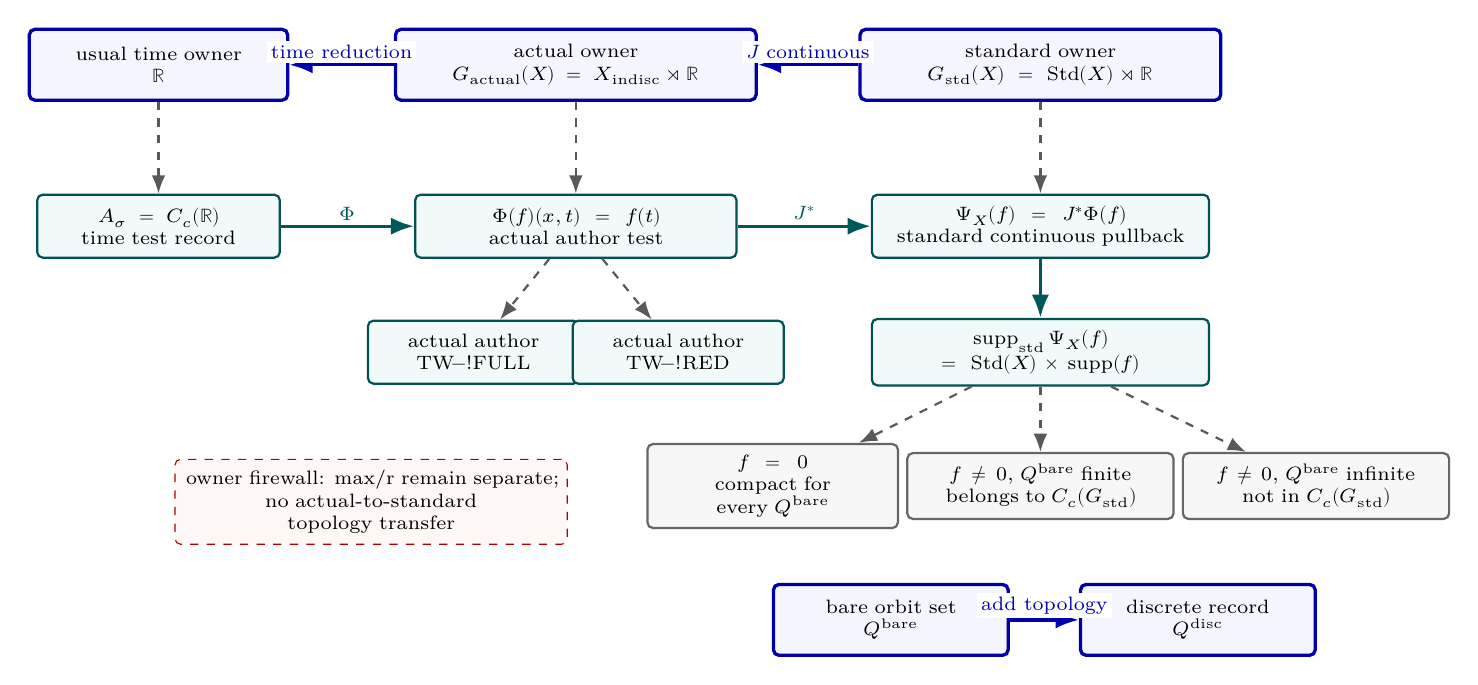
\begin{tikzpicture}[
  font=\scriptsize,
  >=Latex,
  owner/.style={draw=blue!65!black, rounded corners=2pt, very thick,
    fill=blue!4, align=center, minimum height=9mm, inner sep=4pt},
  record/.style={draw=teal!65!black, rounded corners=2pt, thick,
    fill=teal!5, align=center, minimum height=8mm, inner sep=4pt},
  branch/.style={draw=black!60, rounded corners=2pt, thick,
    fill=black!3, align=center, minimum height=8mm, inner sep=4pt},
  guard/.style={draw=red!70!black, dashed, rounded corners=2pt,
    fill=red!3, align=center, inner sep=4pt},
  map/.style={->, very thick, blue!70!black},
  pull/.style={->, very thick, teal!70!black},
  inherit/.style={->, thick, dashed, black!65},
  lab/.style={fill=white, inner sep=1.5pt, align=center}
]
  \node[owner, text width=30mm] (time) at (0,4.4)
    {usual time owner\\$\mathbb R$};
  \node[owner, text width=43mm] (actual) at (5.3,4.4)
    {actual owner\\$G_{\mathrm{actual}}(X)=X_{\mathrm{indisc}}\rtimes\mathbb R$};
  \node[owner, text width=43mm] (standard) at (11.2,4.4)
    {standard owner\\$G_{\mathrm{std}}(X)=\operatorname{Std}(X)\rtimes\mathbb R$};

  \draw[map] (actual) -- node[lab,above]{time reduction} (time);
  \draw[map] (standard) -- node[lab,above]{$J$ continuous} (actual);

  \node[record, text width=28mm] (timerec) at (0,2.35)
    {$A_\sigma=C_c(\mathbb R)$\\time test record};
  \node[record, text width=38mm] (actualrec) at (5.3,2.35)
    {$\Phi(f)(x,t)=f(t)$\\actual author test};
  \node[record, text width=40mm] (stdrec) at (11.2,2.35)
    {$\Psi_X(f)=J^*\Phi(f)$\\standard continuous pullback};

  \draw[pull] (timerec) -- node[lab,above]{$\Phi$} (actualrec);
  \draw[pull] (actualrec) -- node[lab,above]{$J^*$} (stdrec);
  \draw[inherit] (time) -- (timerec);
  \draw[inherit] (actual) -- (actualrec);
  \draw[inherit] (standard) -- (stdrec);

  \node[record, text width=24mm] (maxrec) at (4.0,0.75)
    {actual author\\$\mathrm{TW\!-!FULL}$};
  \node[record, text width=24mm] (redrec) at (6.6,0.75)
    {actual author\\$\mathrm{TW\!-!RED}$};
  \draw[inherit] (actualrec) -- (maxrec);
  \draw[inherit] (actualrec) -- (redrec);

  \node[record, text width=40mm] (support) at (11.2,0.75)
    {$\supp_{\mathrm{std}}\Psi_X(f)$\\$=\operatorname{Std}(X)\times\supp(f)$};
  \draw[pull] (stdrec) -- (support);

  \node[branch, text width=29mm] (zero) at (7.8,-0.95)
    {$f=0$\\compact for every $Q^{\mathrm{bare}}$};
  \node[branch, text width=31mm] (finite) at (11.2,-0.95)
    {$f\ne0$, $Q^{\mathrm{bare}}$ finite\\belongs to $C_c(G_{\mathrm{std}})$};
  \node[branch, text width=31mm] (infinite) at (14.7,-0.95)
    {$f\ne0$, $Q^{\mathrm{bare}}$ infinite\\not in $C_c(G_{\mathrm{std}})$};
  \draw[inherit] (support) -- (zero);
  \draw[inherit] (support) -- (finite);
  \draw[inherit] (support) -- (infinite);

  \node[guard, text width=47mm] (firewall) at (2.7,-1.15)
    {owner firewall: max/r remain separate;\\no actual-to-standard topology transfer};

  \node[owner, text width=27mm] (bare) at (9.3,-2.65)
    {bare orbit set\\$Q^{\mathrm{bare}}$};
  \node[owner, text width=27mm] (disc) at (13.2,-2.65)
    {discrete record\\$Q^{\mathrm{disc}}$};
  \draw[map] (bare) -- node[lab,above]{add topology} (disc);
\end{tikzpicture}
}
\caption{Owner and support directions for the typed comparison.  The diagram
is schematic: it asserts no topology transfer, completion theorem, or
globally named actual twisted groupoid $C^*$-algebra.}
\label{fig:owner-support}
\end{figure}
\FloatBarrier

\section{Normalized twist collapse and author transports}\label{sec:twists}

Paper~12's all-degree factorization theorem gives unique time cochains
$\alpha_0$ and $\sigma_0$ with
\[
 \alpha(x,t)=\alpha_0(t),\qquad
 \Sigma((x,s),(x\mathbin{.}s,t))=\sigma_0(s,t).
\]
This is an inherited premise, not a new factorization result.  Direct
substitution in the range-first nerve formulas shows that normalization,
the cocycle equation, pointwise products, and
$\sigma\overline\tau=\delta\alpha$ commute with pullback and evaluation.
Consequently the actual and time normalized gauge quotients are algebraically
identified, without transferring topology.

For clarity, write an actual degree-two cochain in range-first variables as
$\Sigma(x;s,t)$.  Factorization says $\Sigma(x;s,t)=\sigma_0(s,t)$, while an
actual degree-one cochain is $a(x;t)=\alpha_0(t)$.  The actual normalization
$\Sigma(x;s,0)=\Sigma(x;0,t)=1$ is therefore exactly the time normalization.
The actual cocycle identity on the composable triple
$(x,s),(x\mathbin{.}s,t),(x\mathbin{.}(s+t),u)$ becomes
\[
 \sigma_0(s,t)\sigma_0(s+t,u)
 =\sigma_0(t,u)\sigma_0(s,t+u).
\]
Likewise, the actual coboundary becomes
$\alpha_0(s)\alpha_0(t)\overline{\alpha_0(s+t)}$ with no inverse or source
swap.  These elementary evaluations are the entire typed bridge: Paper~12
owns factorization, while this note checks that the normalized operations
respect it at the frozen convention.

The official abstract of Sorkin advertises continuous real-line multiplier
triviality \citep{Sorkin1978Triviality}.  The following proof is included
because our normalization and the direction in \cref{eq:gauge-direction}
must be checked directly; it is not presented as the original
classification.

\begin{theorem}[Direct collapse at the frozen signs]\label{thm:collapse}
Every continuous normalized $\sigma:\R^2\to\T$ has a continuous normalized
$\alpha:\R\to\T$ such that $\sigma=\delta\alpha$.  Two trivializers differ
by a continuous character of $\R$.
\end{theorem}

\begin{proof}
Lift $\sigma$ uniquely through $e^{i(\cdot)}:\R\to\T$ to a continuous
$q:\R^2\to\R$ with $q(0,0)=0$.  Normalization and connectedness make
$q(s,0)=q(0,t)=0$ exactly.  The lifted cocycle defect is continuous and
$2\pi\Z$-valued on connected $\R^3$, hence zero.  Thus $q$ is a normalized
real cocycle.  Its commutator $b(s,t)=q(s,t)-q(t,s)$ is continuous and
additive in each variable.  The continuous Cauchy equation gives
$b(s,t)=\kappa st$; alternation gives $\kappa=0$, so $q$ is symmetric.

Choose $\rho\in C_c^\infty(\R)$ with $\int\rho=1$, define
$h(s)=\int q(s,u)\rho(u)\,du$, and put $q_1=q-\delta h$.  Then
\[
 q_1(s,t)=\int_{\R}[q(s,t+u)-q(s,u)]\rho(u)\,du
\]
has a jointly continuous second partial derivative.  With
$a(r)=\partial_2q_1(r,0)$, differentiation of the cocycle identity at the
third variable $0$ yields
$\partial_2q_1(s,t)=a(s+t)-a(t)$.  If
$A(t)=\int_0^t a(v)\,dv$, integration gives
$q_1(s,t)=A(s+t)-A(s)-A(t)=\delta(-A)(s,t)$.  Therefore
$q=\delta(h-A)$ and
$\alpha(t)=\exp(i(h(t)-A(t)))$ has the required normalization and sign.
Finally, if $\delta\alpha=\delta\beta$, then
$\chi=\beta/\alpha$ satisfies $\chi(s+t)=\chi(s)\chi(t)$; conversely every
continuous character preserves the trivializer equation.
\end{proof}

On $A_\sigma=C_c(\R)$ use the formulas audited for the usual time group
\citep[pp.~5--6]{Austad2021Spectral}:
\begin{align}
 (f*_{\sigma}g)(t)
   &=\int_{\R}f(u)g(t-u)\sigma(u,t-u)\,du,
   \label{eq:twisted-product}\\
 f^{*_{\sigma}}(t)
   &=\overline{\sigma(t,-t)}\,\overline{f(-t)}.
   \label{eq:twisted-star}
\end{align}
The support inclusion
$\supp(f*_{\sigma}g)\subseteq\supp(f)+\supp(g)$ gives closure.
Absolute Fubini and the cocycle identity give associativity; the inverse-face
identity gives both involution laws.  If
$\sigma\overline\tau=\delta\alpha$, direct cancellation in
\cref{eq:twisted-product,eq:twisted-star} gives
\[
 U_\alpha f(t)=\alpha(t)f(t),\qquad
 U_\alpha(f*_{\sigma}g)=U_\alpha f*_{\tau}U_\alpha g,
 \qquad U_\alpha(f^{*_{\sigma}})=(U_\alpha f)^{*_{\tau}}.
\]

The sign in this gauge identity can be audited without shorthand.  At the
integrand pair $(u,t-u)$, \cref{eq:gauge-direction} is equivalent to
\[
 \alpha(t)\sigma(u,t-u)
 =\alpha(u)\alpha(t-u)\tau(u,t-u),
\]
which is precisely the factor needed on the two inputs to the $\tau$-product.
At the inverse face it yields
$\alpha(t)\overline{\sigma(t,-t)}=
\overline{\tau(t,-t)}\overline{\alpha(-t)}$, precisely the involution
factor.  Circle multiplication changes neither absolute values nor support.
Thus the same identity controls product, star, support, and every later
gauge square.

For associativity, the two iterated integrals are absolutely integrable
because the three functions have compact support.  After a change of
variables places both expressions over $(u,v)$, their scalar factors are
$\sigma(u,v)\sigma(u+v,t-u-v)$ and
$\sigma(v,t-u-v)\sigma(u,t-u)$; the cocycle equation identifies them.
For the star law, normalization and the cocycle identity at inverse faces
give the required conjugate factor.  These verifications occur on
$C_c(\R)$ before any norm or completion is introduced.

The intrinsic projective left regular representation is
\[
 (\lambda_\sigma(s)\xi)(t)=\sigma(s,t-s)\xi(t-s),
 \qquad
 \Lambda_\sigma(f)=\int_{\R}f(s)\lambda_\sigma(s)\,ds.
\]
It satisfies
$\lambda_\sigma(s)\lambda_\sigma(u)=
\sigma(s,u)\lambda_\sigma(s+u)$ and integrates to a
$*$-representation.  Multiplication by the trivializer intertwines it with
the untwisted regular representation.  We define the time maximal and
reduced norms separately and only then use amenability of the usual group
$\R$: Austad's exact endpoint is Proposition~2.4 on printed p.~7, cited
there as a continuous specialization of Leptin's Satz~6 on printed p.~204
\citep{Austad2021Spectral,Leptin1968Darstellungen}.  Hulanicki's
invariant-mean and weak-containment results provide group-level context
\citep[pp.~87--88]{Hulanicki1966Folner}
\citep[visible printed pp.~56--58]{Hulanicki1964WeakContainment}; the latter
bibliography retains the official 27--59 pagination despite the official
scan beginning visibly at p.~37.  None of these sources proves an actual
non-Hausdorff completion.

More explicitly, $M_\alpha\xi(t)=\alpha(t)\xi(t)$ satisfies
$M_\alpha\lambda_\sigma(s)M_{\overline\alpha}
=\alpha(s)\lambda_1(s)$ when $\sigma=\delta\alpha$.  After integration this
is the same oriented gauge as $U_\alpha$.  The reduced norm is
$\lVert\Lambda_\sigma(f)\rVert$; the maximal norm is the supremum over the
audited $L^1$-continuous $*$-representations.  Gauge transport identifies
each norm with its untwisted time counterpart, and amenability identifies
the two time endpoints.  This order is essential: amenability is not
asserted for the actual owner, and equality is not inferred merely from the
existence of a projective representation.

Paper~11 supplies the bijection
\[
 \Phi_X:C_c(\R)\longrightarrow C_{\mathrm{glob}}(\Gactual(X)),
 \qquad \Phi_X(f)(x,t)=f(t),
\]
whose actual support is $X\times\supp(f)$ and is quasi-compact at the actual
owner.  For $\Sigma=\pi_2^*\sigma$, we \emph{define} the twisted author
product, star, and both transported norms through $\Phi_X$.  Hence
\[
 \Phi_X(f)*_\Sigma\Phi_X(g)=\Phi_X(f*_{\sigma}g),
 \qquad
 \Phi_X(f)^{*_{\Sigma}}=\Phi_X(f^{*_{\sigma}}).
\]
The word ``define'' is load-bearing.  The actual topology makes every
continuous separated-target scalar function depend only on time, and
Paper~11 supplies the untwisted author support and completion contracts.
Here we pull the proved time twist through that bijection and do not appeal
to a general non-Hausdorff twisted groupoid construction.  Support remains
$X\times\supp(f)$ because neither a circle gauge nor $\Phi_X$ changes the
zero set in the time variable.  Associativity and both star laws therefore
arrive only after their time formulas have been checked above.

The completed records
$\mathrm{TW\!-!FULL\!-!TRANSPORT}_X(\Sigma)$ and
$\mathrm{TW\!-!RED\!-!TRANSPORT}_X(\Sigma)$ are separate author records,
even though the amenable time endpoint makes their transported norms agree
on the common dense image.  This construction deliberately does not name a
global twisted groupoid $C^*$-algebra on $\Gactual(X)$.

If $\beta$ is another trivializer, then $\chi=\beta/\alpha$ is a continuous
character.  The two untwisted presentations consequently differ by the
character automorphisms $U_\chi$ and $M_\chi$, so the transported normed
records are choice-independent in the stated sense.  This does not select a
preferred trivializer, Fourier coordinate, or orbit origin.  Nor does the
time full/reduced equality license erasing the two author record names: their
separate typing is retained for every later naturality square.

\section{Named nonretention and support transfer}\label{sec:support}

The gauge collapse has a precisely bounded nonretention consequence.  Tags
may record an owner and a chosen multiplier, but after those tags are
forgotten only the four outputs in \cref{tab:nonretention} have a common
value.  This is trace artifact \nolinkurl{P13-TAB-03-NONRETENTION} in the
package README, ``Strict six-key artifact traces.''

\begin{proposition}[Exactly four named constant outputs]\label{prop:four}
Across the registered globally indiscrete right-real action owners, the
tag-forgotten outputs \texttt{TIME-GAUGE}, \texttt{ACTUAL-TW-TEST},
\texttt{ACTUAL-TW-FULL}, and \texttt{ACTUAL-TW-RED} are constant.  No claim
is made about every invariant of the owner.
\end{proposition}

\begin{proof}
\Cref{thm:collapse} makes the time gauge class zero.  The oriented maps
$U_\alpha$ identify the time test records and extend isometrically to the
two separately transported completions.  Conjugating through the Paper~11
maps $\Phi_X$ gives inter-owner test, maximal, and reduced isomorphisms.
These calculations account for exactly the registered rows and no others.
\end{proof}

For two owners $X$ and $Y$, the test-level comparison is explicitly
$\Phi_Y\Phi_X^{-1}$ after both twists have been transported to the common
time record.  The maximal comparison is the unique isometric extension of
that map to the separately named maximal completions; the reduced comparison
is constructed again on the separately named reduced completions.  This is
why the proposition is an inter-owner statement about four registered
outputs rather than a claim that the actions themselves are isomorphic.
Strict equivariant maps are natural because their pullbacks fix every
time-only function $f(t)$.

\begin{table}[H]
\centering
\caption{The exact four-output nonretention statement.}
\label{tab:nonretention}
\small
\begin{tabularx}{\linewidth}{P{0.25\linewidth}YY}
\toprule
Named output & Tag-forgotten value & Mandatory retention \\
\midrule
\texttt{TIME-GAUGE} & zero gauge class & literal owner and cochain tier \\
\texttt{ACTUAL-TW-TEST} & common twisted test $*$-class & actual support convention \\
\texttt{ACTUAL-TW-FULL} & common transported maximal class & maximal label \\
\texttt{ACTUAL-TW-RED} & common transported reduced class & reduced label \\
\bottomrule
\end{tabularx}
\end{table}

If $H_x\subset\R$ is a literal stabilizer, restriction of a globally
trivial multiplier has zero class in the registered restricted continuous
gauge quotient: $(\delta\alpha)|_{H_x}=\delta(\alpha|_{H_x})$.  This does not
erase $H_x$, its embedding, topology, period, clock, or representation
theory.  In the fixed-prime owner, Paper~9 retains
$H=(\log p)\Z$ and period $\log p$; the scalar twist adds no registered
restricted continuous cohomology-class invariant and therefore cannot
recover $p$.

The restriction statement is intentionally cohomological rather than
set-theoretic.  It says that a class represented by $\delta\alpha$ remains a
coboundary after applying the restriction map.  It does not say that the
subgroup $H_x$ becomes trivial, that two embedded lattices are equal, or that
the quotient circle loses its marked period.  In particular, characters of
$H_x$ and representations built from the literal subgroup remain available
even though this one continuous degree-two class vanishes.

We next compare actual quasi-compact support with standard compact support.
For $f\in C_c(\R)$ put $K=\supp(f)$ and
$\Psi_X(f)=J^*\Phi_X(f)$.  Since $J$ is identity on the arrow carrier,
\begin{equation}\label{eq:support-product}
 \supp_{\mathrm{std}}\Psi_X(f)
   =\Std(X)\times K
   =\coprod_{q\in\Qbare}(O_q\times K).
\end{equation}

\begin{theorem}[Zero/finite/infinite support criterion]\label{thm:support}
For a nonempty common-period owner,
\[
 \Psi_X(f)\in C_c(\Gstd(X))
 \quad\Longleftrightarrow\quad
 f=0\ \text{or}\ \Qbare\ \text{is finite}.
\]
If $\Qbare$ is infinite and
$T_X=J^*\Phi_X(C_c(\R))\subset C(\Gstd(X))$, then
\[
 T_X\cap C_c(\Gstd(X))=\{0\}.
\]
Every allowed circle gauge preserves this dichotomy.
\end{theorem}

\begin{proof}
For $f=0$, the support is empty.  If $f\ne0$ and $\Qbare$ is finite,
\cref{eq:support-product} is a finite union of compact sets
$O_q\times K$.  If $\Qbare$ is infinite, the nonempty component sets
$O_q\times K$ form an open cover of the support with no finite subcover, so
the support is not compact.  Injectivity of $\Psi_X$ gives the intersection
statement.  Finally, a circle gauge $\alpha$ is nowhere zero, hence
$\supp(\alpha f)=\supp(f)$.
\end{proof}

Thus \cref{eq:support-product,thm:support} is exactly the support branch
displayed in \cref{fig:owner-support}
\TraceRef{P13-FIG-01-OWNER-SUPPORT}; no topology or completion arrow is
inferred from that schematic.

The product-support formula itself uses no countability.  The nonzero locus
of $\Psi_X(f)$ is
$\Std(X)\times\{t:f(t)\ne0\}$, and for a nonempty space $Z$ one has
$\overline{Z\times E}=Z\times\overline E$ in $Z\times\R$.  This proves
\cref{eq:support-product} directly, including the empty-support case.  On an
infinite coproduct, the component sets $O_q\times K$ are nonempty relatively
open subsets of the support.  Their cover has no finite subcover; no finite
diagnostic, sequence of components, or limiting argument is being used.

For finite $\Qbare$, direct substitution into the standard component
convolution makes $\Psi_X$ an injective $*$-map onto the time-only
unit-coordinate-constant test subalgebra.  This optional finite branch is
only a test-function statement: it yields no norm comparison or completion
map.  For infinite $\Qbare$, the continuous pullback still exists, but no
nonzero time-only actual test function lands in the standard compact-support
test algebra.

\section{Selected component isometries}\label{sec:components}

Fix a compact standard orbit $O_q$ and
$\epsilon\in\{\max,\mathrm r\}$.  On the component test record use
\begin{align*}
 (F*_{\sigma}G)(x,t)
  &=\int_{\R}F(x,u)G(x\mathbin{.}u,t-u)
       \sigma(u,t-u)\,du,\\
 F^{*_{\sigma}}(x,t)
  &=\overline{\sigma(t,-t)}
       \overline{F(x\mathbin{.}t,-t)}.
\end{align*}
For these range-first coordinates the component $I$-norm is
\[
 \lVert F\rVert_I=\max\left\{
 \sup_{x\in O_q}\int_{\R}|F(x,t)|\,dt,
 \sup_{x\in O_q}\int_{\R}|F(x\mathbin{.}t,-t)|\,dt
 \right\}.
\]
The maximal record is the universal completion over $I$-norm-decreasing
test representations.  The reduced record is the completion for the
supremum of the intrinsic unit-regular representations.  If
$\sigma\overline\tau=\delta\alpha$, then
$U_{\alpha,q}F(x,t)=\alpha(t)F(x,t)$ preserves the component product, star,
support, and $I$-norm.  Taking $\tau=1$ transports the component record to
the audited ordinary compact-orbit record without choosing a torsor origin;
it also shows that both proposed completions exist.

The ordinary untwisted component owner is the transformation crossed
product described by Buss--Holkar--Meyer, while Williams supplies the
ordinary universal dense algebra, regular norms, homogeneous-space model,
and amenable-action endpoint \citep[Lemma 2.27, Remarks 2.29--2.30,
Theorem 4.30, and Theorem 7.13]{Williams2007CrossedProducts}.  We do not use
Williams's injective group-valued multiplier map as a $C^*$-faithfulness
proof.  Instead the following chain is direct.

Define the origin-free constant-in-the-unit map
\[
 d_{q,\sigma}:C_c(\R)\longrightarrow C_c(O_q\rtimes\R,\sigma),
 \qquad d_{q,\sigma}(f)(x,t)=f(t).
\]
Its support is $O_q\times\supp(f)$, compact because $O_q$ is compact; hence
it really belongs to the component test algebra.  Substitution shows that it
preserves product and star, and nonemptiness of $O_q$ gives injectivity at
test level.  Notice what is not used: there is no basepoint of $O_q$, no
identification of two different torsors, and no listing of components.  The
map is intrinsic because being constant in the unit variable is preserved by
every equivariant translation.

For the component
reduced norm, its every-unit regular representation is exactly
$\Lambda_\sigma(f)$, so
\begin{equation}\label{eq:reduced-component}
 \lVert d_{q,\sigma}(f)\rVert_{B_{q,\sigma}^{\mathrm r}}
 =\lVert f\rVert_{\cstarred(\R,\sigma)}.
\end{equation}
Here the source fibre at $x$ is intrinsically parameterized by
$t\mapsto(x\mathbin{.}(-t),t)$, and the corresponding regular action is
\[
 [\operatorname{Reg}_{q,x,\sigma}(F)\xi](t)
 =\int_{\R}F(x\mathbin{.}(-t),u)\sigma(u,t-u)
       \xi(t-u)\,du.
\]
Its kernel is bounded by Schur's test using the two terms of the displayed
$I$-norm.  Thus every unit-regular representation is among those dominated
by the maximal norm.  When $F=d_{q,\sigma}(f)$ the coefficient loses its
unit variable and the formula becomes $\Lambda_\sigma(f)$ at every $x$,
which proves the equality in \cref{eq:reduced-component}, not merely one
inequality.

For the maximal norm, every component representation restricted along
$d_{q,\sigma}$ is an $L^1(\R,\sigma)$-continuous $*$-representation;
therefore
\begin{equation}\label{eq:max-component}
 \lVert d_{q,\sigma}(f)\rVert_{B_{q,\sigma}^{\max}}
 \leq \lVert f\rVert_{\cstarmax(\R,\sigma)}.
\end{equation}

The maximal estimate also has the correct direction for a reason.  On the
constant-in-unit image, both terms of the component $I$-norm equal
$\lVert f\rVert_1$.  Therefore restriction of any representation counted by
the component universal norm gives an admissible time representation.  The
time maximal norm is the supremum over all such time representations, so it
dominates the restricted component norm.  Faithfulness cannot be read off
from a canonical group-valued multiplier map; it follows only after this
upper bound is closed against the reduced lower endpoint.

\begin{theorem}[Selected maximal and reduced isometries]\label{thm:component-isometry}
For every $q$, $f\in C_c(\R)$, and separately for
$\epsilon=\max$ and $\epsilon=\mathrm r$,
\[
 \lVert d_{q,\sigma}(f)\rVert_{B_{q,\sigma}^{\epsilon}}
   =\lVert f\rVert_{C^*_{\epsilon}(\R,\sigma)}.
\]
Thus $d_{q,\sigma}$ extends to an isometric faithful $*$-homomorphism
$d_{q,\sigma}^{\epsilon}:C^*_{\epsilon}(\R,\sigma)
\to B_{q,\sigma}^{\epsilon}$ whose image lies in the component algebra.
\end{theorem}

\begin{proof}
Combine \cref{eq:reduced-component,eq:max-component}, domination of reduced
by maximal norm, and amenability only at the time endpoint:
\[
 \lVert f\rVert_{\mathrm{time},\max}
 \geq \lVert d_q(f)\rVert_{\mathrm{component},\max}
 \geq \lVert d_q(f)\rVert_{\mathrm{component},\mathrm r}
 =\lVert f\rVert_{\mathrm{time},\mathrm r}
 =\lVert f\rVert_{\mathrm{time},\max}.
\]
Every inequality is equality.  Completion gives the two isometries
separately.  If $f_n$ converges in the time completion, then
$d_{q,\sigma}(f_n)$ converges inside $B_{q,\sigma}^{\epsilon}$, so the
completed image is not merely a multiplier.
\end{proof}

The theorem identifies only the selected time images.  It gives neither
$B_{q,\sigma}^{\max}=B_{q,\sigma}^{\mathrm r}$ nor a common origin across
components, an orbit enumeration, or a globally named standard twisted
groupoid completion.

Gauge covariance is already present at component level:
$U_{\alpha,q}^{\epsilon}d_{q,\sigma}^{\epsilon}
=d_{q,\tau}^{\epsilon}U_\alpha^{\epsilon}$.  Both sides are first equal on
the dense test algebra and then extend by isometry.  Because no origin was
used in the regular fibre parameterization or in $d_{q,\sigma}$, changing a
temporary presentation $O_q\cong\R/H$ by an equivariant translation fixes
the constant-in-unit image.  These facts will permit a coordinatewise
diagonal without introducing simultaneous identifications among the
components.

The selected-image qualification is substantive.  A general component
function depends on its unit coordinate, so its norm is not tested by the
constant-in-unit restriction alone.  The chain above proves the norm of
$d_{q,\sigma}(f)$ exactly; it says nothing about a complementary subspace or
about whether the canonical maximal-to-reduced quotient is injective on the
entire component algebra.  This is why both superscripts remain present in
the diagonal construction below even though their time inputs have equal
norms.

\section{Generic constant diagonals and typed instantiations}\label{sec:generic}

The next theorem is deliberately generic and occurs only after
\cref{thm:component-isometry}.  It contains no prime, packet, twist, orbit
topology, common origin, or enumeration.

\begin{theorem}[Generic constant-diagonal corona lemma]\label{thm:generic-diagonal}
Let $I$ be a nonempty set, let $C$ and $B_i$ be $C^*$-algebras, and let
$\varphi_i:C\to B_i$ be isometric $*$-homomorphisms.  Put
$A=\bigoplus_{i\in I}^{c_0}B_i$.  Then
\[
 M(A)\cong\prod_{i\in I}^{\mathrm{bounded}}M(B_i),
 \qquad
 \Delta(c)=(\varphi_i(c))_{i\in I}\in M(A)
\]
defines an isometric faithful $*$-homomorphism $\Delta:C\to M(A)$.  Moreover
\[
 \Delta(c)\in A\quad\Longleftrightarrow\quad c=0\ \text{or}\ I\text{ is finite}.
\]
If $I$ is infinite, then
\[
 \lVert\Delta(c)+A\rVert_{M(A)/A}
   =\dist(\Delta(c),A)=\lVert c\rVert,
\]
so the corona composite is isometric and faithful.
\end{theorem}

Recall that an arbitrary-index $c_0$ sum means
\[
 A=\left\{(b_i):\sup_i\lVert b_i\rVert<\infty,
 \ \{i:\lVert b_i\rVert\geq\eta\}\text{ is finite for every }\eta>0
 \right\}.
\]
This definition does not ask that $I$ be countable or enumerated.  It also
shows why the multiplier product in \cref{thm:generic-diagonal} must not be
substituted for $A$: the bounded product is the multiplier algebra, while
the $c_0$ condition continues to define the essential ideal.

\begin{proof}
Realize a multiplier of $A$ as a double centralizer $(L,R)$.  Orthogonality
of distinct coordinate ideals, tested against approximate identities,
forces $(L,R)$ to preserve every $B_i$.  Restriction gives a uniformly
bounded family $(m_i)\in\prod_i M(B_i)$.  Conversely, a uniformly bounded
family acts coordinatewise on $A$ and preserves the condition that norms
vanish at infinity.  These assignments are inverse, and testing on a single
coordinate shows that their norm is $\sup_i\lVert m_i\rVert$.

Since every $\varphi_i$ is isometric,
$\sup_i\lVert\varphi_i(c)\rVert=\lVert c\rVert$.  A constant-norm family is
$c_0$ precisely when it is zero or the index set is finite.  If $I$ is
infinite and $b=(b_i)\in A$, then for every $\eta>0$ only finitely many
$i$ satisfy $\lVert b_i\rVert\geq\eta$.  Choose an index outside that set;
then
$\lVert\varphi_i(c)-b_i\rVert\geq\lVert c\rVert-\eta$.  Taking the
supremum, then $\eta\downarrow0$, gives the lower bound for the distance;
$b=0$ gives the reverse bound.
\end{proof}

The theorem separates a reusable operator-algebra fact from every later
owner label.  In particular, the equality of the quotient norm is proved by
distance to the $c_0$ ideal, not inferred from the bare assertion that a
class is nonzero.  The zero, finite-index, and infinite-index cases are all
part of the same generic statement.

That generic theorem, including its zero/finite/infinite branches and the
subsequent separately typed maximal/reduced instantiations, is diagrammed in
\cref{fig:generic-diagonal}.  The reverse trace artifact is
\nolinkurl{P13-FIG-02-GENERIC-DIAGONAL}.  Its locator is the package README,
``Strict six-key artifact traces.''

\begin{figure}[t]
\centering
\resizebox{\linewidth}{!}{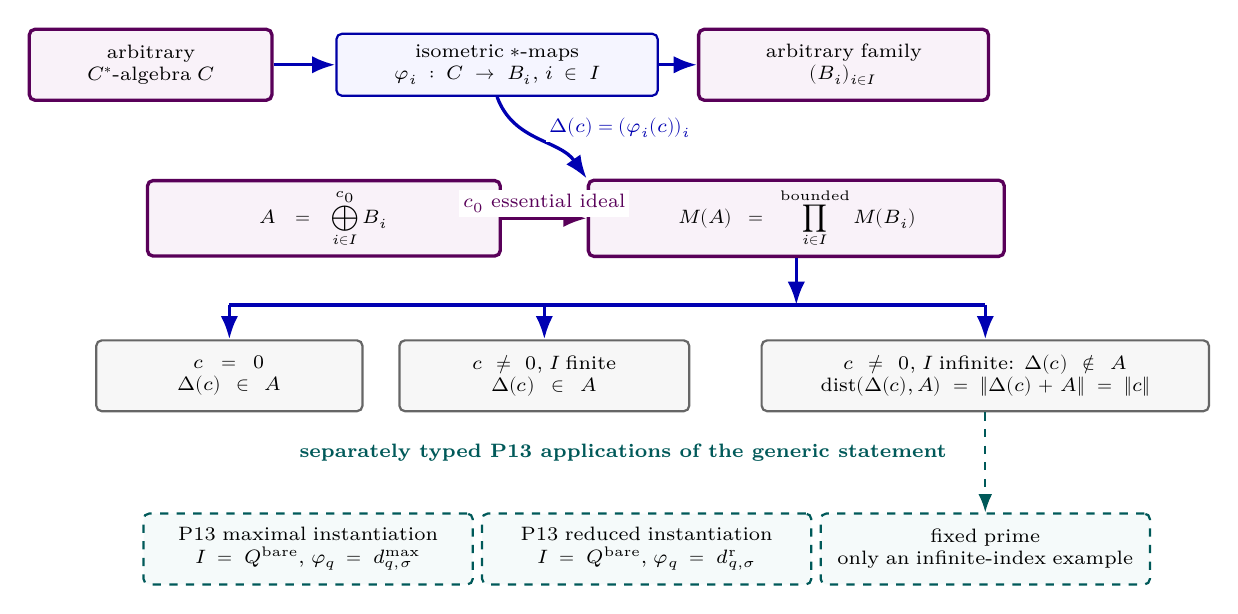
\begin{tikzpicture}[
  font=\scriptsize,
  >=Latex,
  algebra/.style={draw=violet!70!black, rounded corners=2pt, very thick,
    fill=violet!5, align=center, minimum height=9mm, inner sep=4pt},
  mapbox/.style={draw=blue!65!black, rounded corners=2pt, thick,
    fill=blue!4, align=center, inner sep=4pt},
  branch/.style={draw=black!60, rounded corners=2pt, thick,
    fill=black!3, align=center, minimum height=9mm, inner sep=4pt},
  p13/.style={draw=teal!70!black, rounded corners=2pt, thick, dashed,
    fill=teal!4, align=center, minimum height=9mm, inner sep=4pt},
  map/.style={->, very thick, blue!70!black},
  inclusion/.style={->, very thick, violet!70!black},
  inst/.style={->, thick, dashed, teal!70!black},
  lab/.style={fill=white, inner sep=1.5pt, align=center}
]
  \node[algebra, text width=28mm] (C) at (0,4.5)
    {arbitrary\\$C^*$-algebra $C$};
  \node[mapbox, text width=38mm] (phis) at (4.4,4.5)
    {isometric $*$-maps\\$\varphi_i:C\to B_i$, $i\in I$};
  \node[algebra, text width=34mm] (Bi) at (8.8,4.5)
    {arbitrary family\\$(B_i)_{i\in I}$};
  \draw[map] (C) -- (phis);
  \draw[map] (phis) -- (Bi);

  \node[algebra, text width=42mm] (A) at (2.2,2.55)
    {$A=\displaystyle\bigoplus_{i\in I}^{c_0}B_i$};
  \node[algebra, text width=50mm] (MA) at (8.2,2.55)
    {$M(A)=\displaystyle\prod_{i\in I}^{\mathrm{bounded}}M(B_i)$};
  \draw[inclusion] (A) -- node[lab,above]{$c_0$ essential ideal} (MA);
  \draw[map] (phis.south) to[out=-70,in=125]
    node[lab,pos=.56,above right]{$\Delta(c)=(\varphi_i(c))_i$} (MA.north west);

  \node[branch, text width=31mm] (zero) at (1.0,0.55)
    {$c=0$\\$\Delta(c)\in A$};
  \node[branch, text width=34mm] (finite) at (5.0,0.55)
    {$c\ne0$, $I$ finite\\$\Delta(c)\in A$};
  \node[branch, text width=54mm] (infinite) at (10.6,0.55)
    {$c\ne0$, $I$ infinite: $\Delta(c)\notin A$\\
     $\dist(\Delta(c),A)=\lVert\Delta(c)+A\rVert=\lVert c\rVert$};
  \coordinate (split) at (8.2,1.45);
  \draw[map] (MA.south) -- (split);
  \draw[blue!70!black,very thick] (zero.north |- split) -- (infinite.north |- split);
  \draw[map] (zero.north |- split) -- (zero.north);
  \draw[map] (finite.north |- split) -- (finite.north);
  \draw[map] (infinite.north |- split) -- (infinite.north);

  \node[font=\scriptsize\bfseries,text=teal!70!black] at (6.0,-0.42)
    {separately typed P13 applications of the generic statement};
  \node[p13, text width=39mm] (max) at (2.0,-1.65)
    {P13 maximal instantiation\\$I=Q^{\mathrm{bare}}$, $\varphi_q=d_{q,\sigma}^{\max}$};
  \node[p13, text width=39mm] (red) at (6.3,-1.65)
    {P13 reduced instantiation\\$I=Q^{\mathrm{bare}}$, $\varphi_q=d_{q,\sigma}^{\mathrm r}$};
  \node[p13, text width=39mm] (prime) at (10.6,-1.65)
    {fixed prime\\only an infinite-index example};
  \draw[inst] (infinite) -- (prime);
\end{tikzpicture}
}
\caption{Generic constant-diagonal lemma and its separately typed
maximal/reduced P13 instantiations.  The fixed-prime owner is only an
infinite-index example; the diagram asserts no owner-specific obstruction,
prime selection, or whole-corona classification.}
\label{fig:generic-diagonal}
\end{figure}

Now take $I=\Qbare$, $C=C^*_{\epsilon}(\R,\sigma)$, and
$\varphi_q=d_{q,\sigma}^{\epsilon}$ from
\cref{thm:component-isometry}.  The resulting isometry is
\[
 D_\sigma^{\epsilon}:C^*_{\epsilon}(\R,\sigma)
 \longrightarrow M(A_{\mathrm{std},\sigma}^{\epsilon}),
 \qquad
 D_\sigma^{\epsilon}(a)=(d_{q,\sigma}^{\epsilon}(a))_q.
\]
For the actual author record with $\Sigma=\pi_2^*\sigma$, let
$\widehat\Phi_{X,\Sigma}^{\epsilon}$ be the completed Paper~11 transport and
define only the named comparison
\[
 \Delta_{X,\Sigma}^{\epsilon}
   =D_\sigma^{\epsilon}\circ
     (\widehat\Phi_{X,\Sigma}^{\epsilon})^{-1}.
\]
This is a map from the named actual author record to the multiplier of the
componentwise standard record; it creates no additional global completion.

The finite and infinite branches now follow without owner-specific
argument.  If $\Qbare$ is finite, every diagonal lies in the $c_0$ sum and
its corona image is zero.  If $\Qbare$ is infinite, a nonzero diagonal has
the same positive norm in every coordinate, so it misses the $c_0$ sum and
survives isometrically in the corona.  This completed dichotomy is the exact
analogue of the test-support split in \cref{thm:support}, but neither theorem
is used as a proof of the other.

If $\sigma\overline\tau=\delta\alpha$, the component gauges assemble
coordinatewise to
$\mathcal U_\alpha^{\epsilon}:A_{\mathrm{std},\sigma}^{\epsilon}
\to A_{\mathrm{std},\tau}^{\epsilon}$, extend to multipliers, and descend to
coronas.  On test functions both sides equal $\alpha(t)f(t)$, so
\begin{align*}
 M(\mathcal U_\alpha^{\epsilon})D_\sigma^{\epsilon}
   &=D_\tau^{\epsilon}U_\alpha^{\epsilon},\\
 M(\mathcal U_\alpha^{\epsilon})\Delta_{X,\pi_2^*\sigma}^{\epsilon}
   &=\Delta_{X,\pi_2^*\tau}^{\epsilon}
       \widehat U_{\alpha,X}^{\epsilon}.
\end{align*}
The same squares commute after quotienting.  Different trivializers differ
by character automorphisms, so membership and corona norms are independent
of that choice.

For a rational prime $p$, Paper~9 supplies the bare fixed-prime set
$Q_p^{\mathrm{bare}}=U_p/H_p$ and Paper~2 supplies its hard continuum lower
bound.  This note adds only the elementary upper closure: there are
countably many coordinates, each of cardinal at most $2^{\aleph_0}$, hence
$|U_p|\leq(2^{\aleph_0})^{\aleph_0}=2^{\aleph_0}$.  Thus
\[
 |Q_p^{\mathrm{bare}}|=2^{\aleph_0}.
\]
The actual quotient $Q_p^{\mathrm{actual}}$ remains indiscrete and second
countable.  Only the discrete record, standard coproduct, and standard arrow
space acquire the corresponding non-second-countability and
non-$\sigma$-compactness consequences.  Those are direct coproduct
consequences, not topology transferred from the actual quotient.

Indeed, the standard components are pairwise disjoint nonempty open sets,
so a countable base cannot distinguish continuum many of them.  Every
compact subset of a coproduct meets only finitely many components, because
the component opens cover it; consequently a countable union of compact
subsets meets at most countably many components.  This proves the stated
non-second-countability and non-$\sigma$-compactness directly for the
standard and discrete records while leaving the actual quotient unchanged.

\begin{corollary}[Fixed-prime nonselective instantiation]\label{cor:prime}
For every rational prime $p$, every continuous normalized $\sigma$, both
$\epsilon=\max$ and $\epsilon=\mathrm r$, and every
$a\in C^*_{\epsilon}(\R,\sigma)$,
\[
 D_{p,\sigma}^{\epsilon}(a)\in
 A_{\mathrm{std},p,\sigma}^{\epsilon}
 \quad\Longleftrightarrow\quad a=0,
 \qquad
 \lVert D_{p,\sigma}^{\epsilon}(a)+A_{\mathrm{std},p,\sigma}^{\epsilon}\rVert
 =\lVert a\rVert.
\]
The analogous statements hold for the named actual author map
$\Delta_{\Gamma_p,\Sigma}^{\epsilon}$ and are gauge covariant.
\end{corollary}

\begin{proof}
The inherited cardinality makes $Q_p^{\mathrm{bare}}$ infinite.  Apply the
generic \cref{thm:generic-diagonal} separately to the two isometric families
proved in \cref{thm:component-isometry}, then compose with the actual author
transport.
\end{proof}

The result is unconditional for each fixed prime and both completion types,
but nonselective: every prime enters the same infinite-index branch.  It
cannot recover $p$ or $\log p$ and supplies no trace, determinant, zeta,
analytic continuation, or spectral operator.

\section{Controls, Route, and limitations}\label{sec:controls}

The frozen replacement diagnostics passed 176 of 176 tests and produced
12 CSV files with 2,665 body rows, including 67 negative controls.  The
receipt covers 13 generated artifacts including the manifest, two fresh
generations, and three byte-identical copies.  These computations were not
rerun during composition.  They check finite sign, support, owner, gauge,
and policy cases; they do not prove continuum cardinality, an arbitrary-index
multiplier identity, the component norm chain, or corona faithfulness.

The reported tuple is the independently reviewed replacement run.  A
historical first-run implementation finding is not smuggled into the note as
current evidence: the replacement generator, tests, reproduction script,
manifest, and outputs were the tuple that received the effective
zero-finding review.  Serialization matters here as well.  Because the
composition gate forbids an unsolicited rerun, this manuscript reports the
frozen receipt and does not compete for a supposed second execution of the
control lane.

No control row is used as a scholarly citation or as a substitute for a
proof locator.

The independent Route audit contains ten Route-A owner records: three are
exploratory and seven rejected.  Every A2, A3, and A4 coordinate fails;
every determinant convention has the exact status
\[
 \texttt{NONE\_BY\_DESIGN\_NO\_DETERMINANT\_OBJECT},
\]
and Route B is false.
Exploratory status records only a limited source relation, not determinant,
spectral, or quantization evidence.  The dated external comparison supports
only the bounded phrase
\[
 \texttt{SUPPORTED\_WITHIN\_SEARCH}
\]
at the 15 August 2026 cutoff; it proves no firstness, priority, or
standalone weight.

\begin{table}[t]
\centering
\caption{Evidence layers and their exact limitations.}
\label{tab:limitations}
\small
\begin{tabularx}{\linewidth}{P{0.17\linewidth}YY}
\toprule
Layer & What it supports & What it cannot support \\
\midrule
Mathematical proof & sign-exact collapse, support criterion, selected
isometries, generic diagonal and typed instances & topology transfer,
whole-algebra equality, full-corona classification, prime selection \\
Finite controls & regression, negative examples, manifest and owner-policy
checks & continuum, arbitrary-index, norm, or faithfulness theorems \\
Route audit & three exploratory and seven rejected owner dispositions & A2,
A3, A4, determinant, zeta, spectral object, or Route-B promotion \\
Source search & no exact package match in the bounded search & absence,
novelty, priority, or standalone status \\
\bottomrule
\end{tabularx}
\end{table}

The remaining boundary is explicit.  We name no global actual twisted
groupoid $C^*$-algebra; transfer no topology among actual, bare, standard,
and discrete records; classify no full corona; and obtain no prime-sensitive
invariant, trace, determinant, zeta object, analytic continuation,
quantization, Hilbert--P\'olya operator, or Route-B object.  A literal
stabilizer and its period remain even when the restricted gauge class is
zero.

Mathematical proof, diagnostic execution, and Route policy are therefore
three noninterchangeable evidence layers.  A green regression row cannot
replace an infinite-index argument; an exploratory Route status cannot turn
a generic diagonal into a determinant; and a correct theorem cannot repair
the retained standalone-positioning finding.  \Cref{tab:limitations}
\TraceRef{P13-TAB-04-LIMITATIONS} records this separation so that later
editing cannot collapse the layers into a single ``pass'' label.

\section{Conclusion}\label{sec:conclusion}

This Technical Note has one practical purpose: to make a chain of valid
facts usable without changing their owners.  The real-line twist collapses
at the frozen gauge sign by a direct phase-lift and smoothing proof, and the
resulting gauge maps transport the time test, maximal, and reduced records to
the separately named actual author records.  Four, and only four, registered
tag-forgotten outputs are constant.  Actual-to-standard pullback has the
exact product-support formula, whose zero/finite/infinite split explains why
an infinite standard coproduct contains no nonzero time-only compactly
supported pullback.

The gain is precision rather than promotion: each arrow, norm, and quotient
is now attached to the record on which it was actually proved.

The analytic order matters.  Reduced and maximal component bounds are proved
separately, amenability is used only at the usual time-group endpoint, and
the resulting isometries concern selected time images rather than whole
component algebras.  Only after those isometries does the corona argument
appear, as a reusable generic constant-diagonal lemma for arbitrary
$c_0$-sums.  The actual-author and fixed-prime statements are typed
instantiations of that lemma.  Their exact norm is useful bookkeeping, but
their uniformity across primes is also their sharp limitation: they recover
no arithmetic parameter.

That generic reduction is why the mathematics closes and why the retained
standalone status does not change.  The NOTE branch remains selected and
\texttt{STANDALONE\_PASS=false}.  Finite controls and Route records support
diagnosis and scope discipline only.  Nothing here promotes the actual owner
to an unaudited completion framework or constructs a trace, determinant,
zeta function, analytic continuation, quantization, or spectral operator.

\section*{Declarations and integrity status}

\noindent\textbf{Author information, affiliations, correspondence, and
CRediT roles:} \AuthorConfirm.

\noindent\textbf{Funding, competing interests, and acknowledgments:}
\AuthorConfirm; no ``none'' declaration is inferred from silence.

\noindent\textbf{Data and code availability:} Local deterministic-control
artifacts and reproduction scripts exist.  Public repository coordinates,
immutable tag, archive accession, DOI, and licences are \AuthorConfirm.

\noindent\textbf{Ethics and consent:} The audited scope contains
mathematical proof and deterministic finite controls, with no identified
human, animal, or sensitive participant data.  Venue-specific ethics and
consent wording, including whether ``not applicable'' is accepted, is
\AuthorConfirm.

\noindent\textbf{Tool assistance and responsibility:} A tool-assisted
research and composition workflow occurred; an AI system is not an author or
mathematical authority.  Venue-compliant disclosure wording and signed human
responsibility for every claim and citation are \AuthorConfirm.

\bibliographystyle{plainnat}
\bibliography{references}

\end{document}
